\begin{figure}[t]
\centering
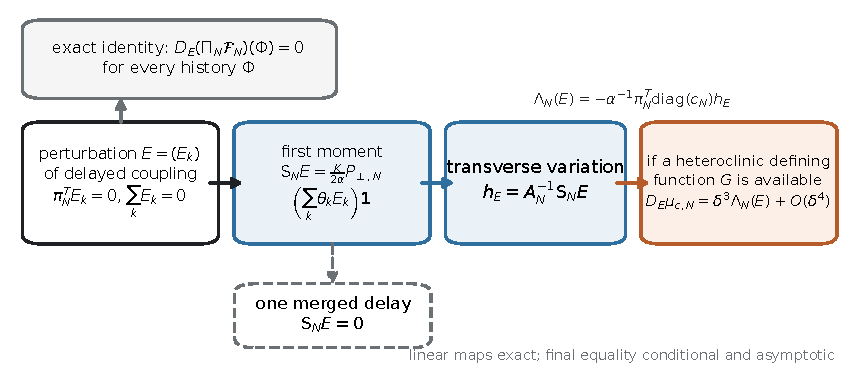
\includegraphics[width=\textwidth]{figures/delay-moment-map.pdf}
\caption{A perturbation of the delayed-coupling matrices satisfying
\(\pi_N^TE_{k,N}=0\) and \(\sum_kE_{k,N}=0\) has zero derivative after
stationary projection at every history.  Its first delay moment can
nevertheless enter the network-mean-zero equation.  The bounded transverse inverse
and the collective Fredholm functional give \(\Lambda_N\).  For any defining
function for a codimension-one heteroclinic condition satisfying the hypotheses of
\cref{thm:fredholm-heteroclinic-sensitivity}, this is the leading derivative
of its connection parameter.  With one merged delay, the first-moment map
vanishes on this perturbation space.  The displayed linear maps are exact;
the connection statement is conditional and asymptotic, and the layout is
schematic.}
\label{fig:delay-moment-map}
\end{figure}
